% Figure for the flipbook of strategies over time

\begin{figure}
\center

	\begin{subfigure}[t]{0.3\textwidth}
	\centering
	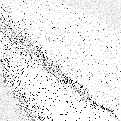
\includegraphics[width=\stratgraphwidth]{images/findings/round2/flipbook/winner/checkpoint_000000.png}
	\caption{Starting Weights}
	\end{subfigure}
	~
	\begin{subfigure}[t]{0.3\textwidth}
	\centering
	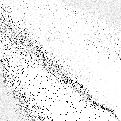
\includegraphics[width=\stratgraphwidth]{images/findings/round2/flipbook/winner/checkpoint_200000.png}
	\caption{After 200,000 games played}
	\end{subfigure}
	~
	\begin{subfigure}[t]{0.3\textwidth}
	\centering
	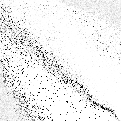
\includegraphics[width=\stratgraphwidth]{images/findings/round2/flipbook/winner/checkpoint_400000.png}
	\caption{After 400,000 games played}
	\end{subfigure}

	\begin{subfigure}[t]{0.3\textwidth}
	\centering
	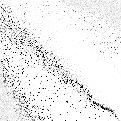
\includegraphics[width=\stratgraphwidth]{images/findings/round2/flipbook/winner/checkpoint_600000.png}
	\caption{After 600,000 games played}
	\end{subfigure}
	~
	\begin{subfigure}[t]{0.3\textwidth}
	\centering
	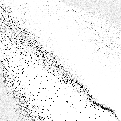
\includegraphics[width=\stratgraphwidth]{images/findings/round2/flipbook/winner/checkpoint_800000.png}
	\caption{After 800,000 games played}
	\end{subfigure}
	~
	\begin{subfigure}[t]{0.3\textwidth}
	\centering
	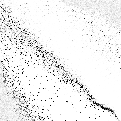
\includegraphics[width=\stratgraphwidth]{images/findings/round2/flipbook/winner/checkpoint_999999.png}
	\caption{Final Weights}
	\end{subfigure}

\caption{
	Training weights representation for a winners' bracket agent's \handmaxavg\
	strategy when the agent is the pone
	over the course of the one million games of Round 2.
	Note that the starting weights are carried over from Round 1,
	so the total training epochs to reach each position is actually
	one million higher than expressed.
}
\label{fig:r2-flip-winner}
\end{figure}
